\documentclass[]{IEEEtran}
% some very useful LaTeX packages include:
%\usepackage{cite}      
\usepackage{graphicx}   
\usepackage{subfigure} 
\usepackage{url}       
\usepackage{amsmath}    
\usepackage{caption2}
% Your document starts here!
\begin{document}

% Define document title and author
	\title{Weekly Report}
	\author{Adviser: Prof. Yang Wen \\Student: Cheng Wensheng\\ Period: 2018.4.2-4.8
	}
	\markboth{Visual Information Processing Group}{}
	\maketitle

% Write abstract here
\begin{abstract}
	This week I mainly put my effort on image annotation tools and reading papers.
\end{abstract}

% Each section begins with a \section{title} command
\section{Image Annotation}
	% \PARstart{}{} creates a tall first letter for this first paragraph
	\PARstart{T}{o} fulfill CETC 54 poject's requirements, we need to add the image annotation function, including detection and segmentation, to the main framework.
	\begin{itemize}
		\item We searched widely on the Internet. There are numerous relevant softwares, like LabelImg, Sloth, Vatic, etc. Nevertheless, most of them can only draw rectangles, and limited to image detection task. Only LabelMe can mark polygons, so can be used in image segmentation task.
		\item We tried various versions of LabelMe, none of them can draw rotation rectangles directly. So we plan to use polygon to draw approximate rotation rectangles, then get accurate rectangles using minimum bounding rectangle.
	\end{itemize}

% Main Part
\section{Classic Paper}
	% LaTeX takes complete care of your document layout ...
	Fully Convolulutional Networks(FCN) launched the new era of semantic segmentation. Most recent papers are motivated by that, so I read this to get some insight into FCN-based methods.
	\begin{itemize}
		\item The authors came up with Fully Convolutional Networks. Their key insight is to replace the last FC layers with upsampling/deconvolution layers. They show that convolutional networks by themselves, trained end-to-end, pixels-to-pixels, improve on the previous best result in semantic segmentation. 
		\item Besides upsampling layers, they define a skip
		architecture that combines semantic information from a deep, coarse layer with appearance information from a shallow, fine layer to produce accurate and detailed segmentations. Fig.~\ref{fig:fcn} is the FCN architecture. Fig.~\ref{fig:result} is part of the results.
	\end{itemize}
\newpage
\begin{figure}[!hbt]
%		 Center the figure.
		\vspace{0.3cm}
%		\hspace{50cm}
		\begin{center}
			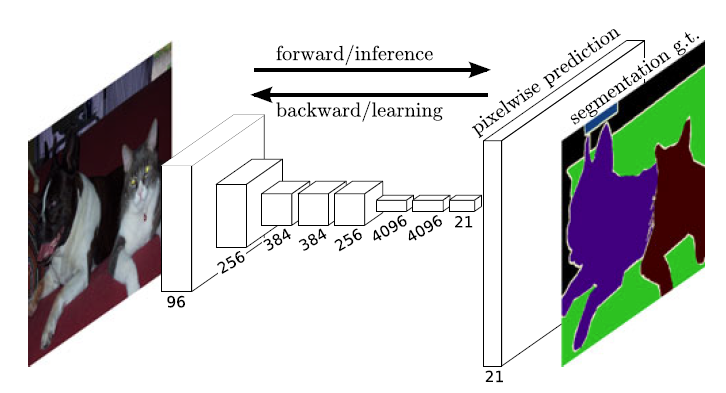
\includegraphics[width=\columnwidth]{fcn}
				%		 Create a subtitle for the figure.
			\caption{FCNs architecture}
			\label{fig:fcn}
		    \hspace{0.5cm}
			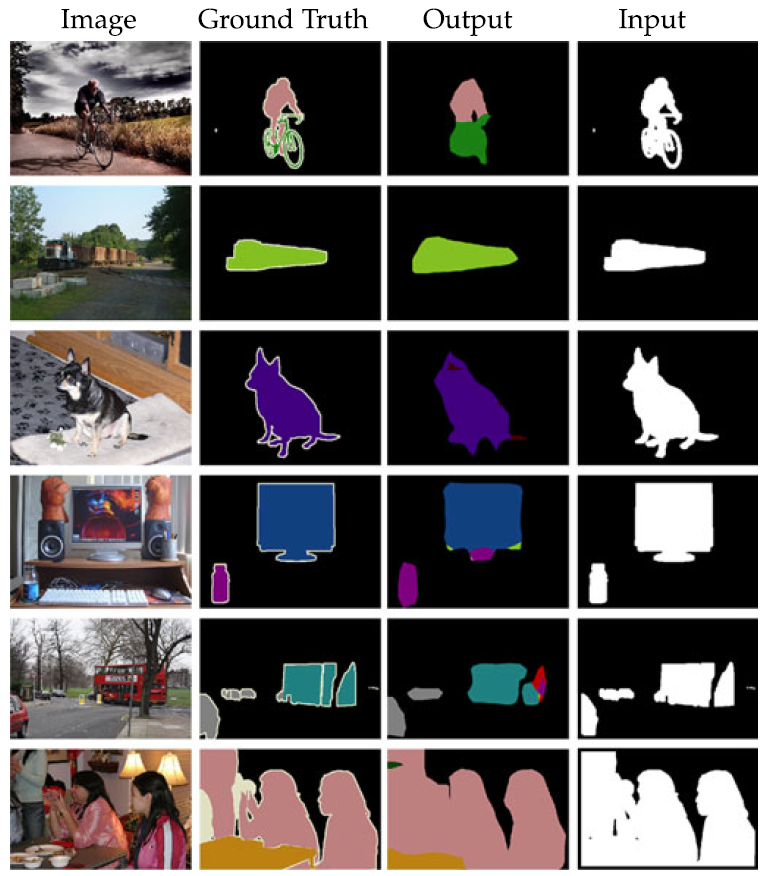
\includegraphics[width=\columnwidth]{result}
				%Create a subtitle for the figure.
			\caption{FCNs semantic segmentation results}
			\label{fig:result}
		\end{center}
	\end{figure}

% Now we need a bibliography:
%\begin{thebibliography}{5}
%
%	%Each item starts with a \bibitem{reference} command and the details thereafter.
%	\bibitem{HOP96} % Transaction paper
%	J.~Hagenauer, E.~Offer, and L.~Papke. Iterative decoding of binary block
%	and convolutional codes. {\em IEEE Trans. Inform. Theory},
%	vol.~42, no.~2, pp.~429–-445, Mar. 1996.
%
%	\bibitem{MJH06} % Conference paper
%	T.~Mayer, H.~Jenkac, and J.~Hagenauer. Turbo base-station cooperation for intercell interference cancellation. {\em IEEE Int. Conf. Commun. (ICC)}, Istanbul, Turkey, pp.~356--361, June 2006.
%
%	\bibitem{Proakis} % Book
%	J.~G.~Proakis. {\em Digital Communications}. McGraw-Hill Book Co.,
%	New York, USA, 3rd edition, 1995.
%
%	\bibitem{talk} % Web document
%	F.~R.~Kschischang. Giving a talk: Guidelines for the Preparation and Presentation of Technical Seminars.
%	\url{http://www.comm.toronto.edu/frank/guide/guide.pdf}.
%
%	\bibitem{5}
%	IEEE Transactions \LaTeX and Microsoft Word Style Files.
%	\url{http://www.ieee.org/web/publications/authors/transjnl/index.html}
%
%\end{thebibliography}

% Your document ends here!
\end{document}